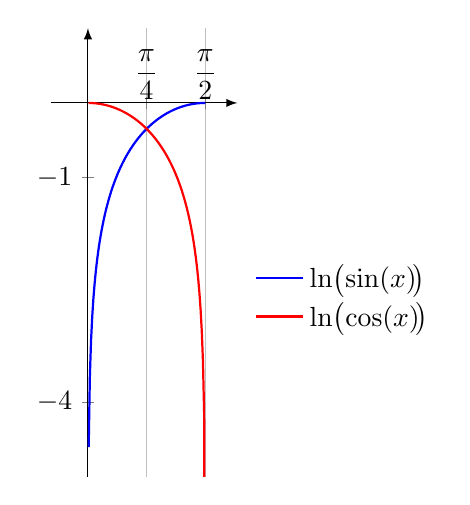
\begin{tikzpicture}
\begin{axis}[
    unit vector ratio*=1 1 1,
    xlabel={},
    ylabel={},
    xmin=-0.5, xmax=2,
    ymin=-5, ymax=1,
    xtick={0,0.7854,1.5708}, 
    xticklabel style={above},
    xticklabels={$0$,$\displaystyle \frac{\pi}{4}$,$\displaystyle \frac{\pi}{2}$},
    ytick={-1,-4},
    yticklabels={$-1$, $-4$},
    xmajorgrids,
    axis lines=middle,
    axis line style={-latex},
    samples=100,
    legend style={
            at={(1.5708,0.5)},
            anchor=north,
            legend cell align=left,
            draw=none % Unterdrücke Box
        },
]

\addplot[blue,thick, domain=0.01:1.5708] {ln(sin(deg(x)))};
\addplot[red,thick, domain=0.01:1.5708] {ln(cos(deg(x)))};
\legend{$\ln\!\big(\!\sin(x)\!\big)$, $\ln\!\big(\!\cos(x)\!\big)$}

\end{axis}
\end{tikzpicture}
